\chapter{Case~Study: Fourth~Year~Project~System}

\todo{Fill this in}

\sectionnote {BM}
\section {Overview}

The fourth-year project management system is used by the department of Systems and Computer Engineering at Carleton University to manage the completion of fourth-year projects by students in software- and systems-related programs. The system is provides students with information on candidate projects, expectations, deadlines and deliverables, and also manages the submission of some project deliverables. The system is used by
\begin{itemize}
\item the \keyword{Project Coordinator}, who is an instructor responsible for overall administration of the fourth-year projects and events;
\item \keyword{Project Supervisors}, which are instructors who suggest candidate projects and supervise the completion of individual projects; and
\item \keyword{Project Group Members}, which are students who must be members of exactly one project group.
\end{itemize}

The system fulfills its functional requirements, but requires significant effort on the part of students to navigate, as all actions, information and deadlines are available at all times. It offers a good example of a system where the user experience could be improved by structuring the system into workflows. Additionally, the system involves deadlines and collaborative activities between multiple actors, which makes it a good test of the capabilities of the Stonepath workflow framework.

\sectionnote {BM}
\section {Requirements}
\label {sec:4ys-requirements}
The required functionality of the fourth-year project management system can be split into three main concerns:
\begin{itemize}
\item \keyword{account management}, which involves creating accounts for Project Supervisors and Project Group Members, as well as authentication with the system;
\item \keyword{project selection}, which entails Project Supervisors creating candidate projects and managing group membership, as well as Project Group Members browsing available projects, consulting with Project Supervisors to find a project, and joining a project; and
\item \keyword{project execution}, which involves all of the collaboration between Project Group Members and the Project Supervisor(s) for their project.
\end{itemize}

Individual use cases for these concerns are illustrated in Figures \ref{fig:case-4ys-use-case-account-management} through \ref{fig:case-4ys-use-case-oral-reports}. Note that the project execution concern has been split into its own use case diagram (Figure \ref{fig:case-4ys-use-case-oral-reports}) as its requirements are somewhat more complex than the other phases of the project lifecycle.

\begin{figure}[!ht]
\centering 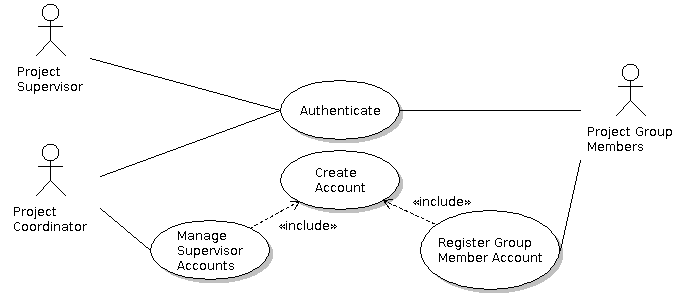
\includegraphics[width=6in]{./img/case-study-fourth-year-system/setup-and-provisioning}
\caption{Use case diagram for the account management functionality of the fourth-year project management system.}
\label{fig:case-4ys-use-case-account-management}
\end{figure}

\begin{figure}[!ht]
\centering 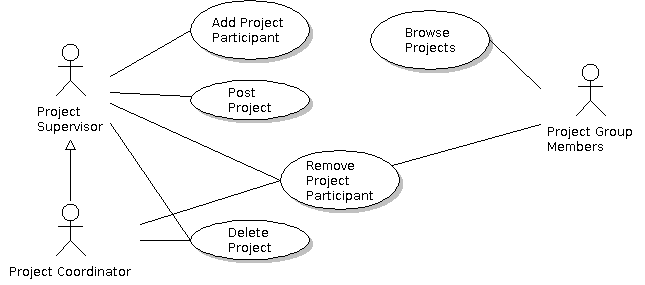
\includegraphics[width=6in]{./img/case-study-fourth-year-system/project-selection}
\caption{Use case diagram for the project selection functionality of the fourth-year project management system.}
\label{fig:case-4ys-use-case-project-selection}
\end{figure}

\begin{figure}[!ht]
\centering 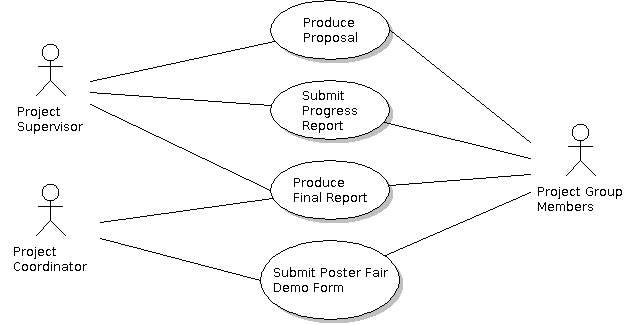
\includegraphics[width=6in]{./img/case-study-fourth-year-system/project-lifecycle}
\caption{Use case diagram for the project execution functionality of the fourth-year project management system. Note that functions related to oral presentations are broken out in Figure \ref{fig:case-4ys-use-case-oral-reports} instead.}
\label{fig:case-4ys-use-case-project-lifecycle}
\end{figure}

\begin{figure}[!ht]
\centering 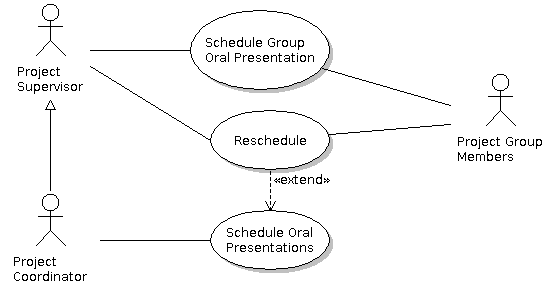
\includegraphics[width=6in]{./img/case-study-fourth-year-system/oral-report-scheduling}
\caption{Use case diagram for the oral presentation functionality of the fourth-year project management system.}
\label{fig:case-4ys-use-case-oral-reports}
\end{figure}


\FloatBarrier

\sectionnote{BM}
\subsection{Project Execution}
\label{sec:4ys-project-execution}

Though all three concerns are important to the system, the most interesting from the point of view of a workflow framework is the project execution phase. This phase accounts for the majority of the lifetime of a fourth-year project, and is also the area in the existing fourth year project management system that could use the most improvement. While account creation and project selection mostly involve basic CRUD (create, read, update, and delete) actions, the execution phase has a well-defined flow:
\begin{enumerate}
\item First, a project proposal must be drafted, submitted, revised, and accepted.
\item After the proposal is accepted, an oral presentation scheduling form must be filled out.
\item Concurrently with scheduling an oral presentation, a progress report must be prepared and submitted.
\item After the progress report is accepted, an oral presentation must be given.
\item After the oral presentation, the group must prepare a presentation for the poster fair. Though this activity has no online deliverables, the group may opt to fill out a poster fair demo request form.
\item While the group is preparing for the poster fair, a final report must also be drafted, submitted, revised, and accepted.
\end{enumerate}
Additionally, each step of the fourth-year project process has associated deadlines.

Use case descriptions for the project execution phase are provided in Tables \ref{tbl:use-case-produce-proposal} through \ref{tbl:use-case-final-report}.

\begin{table}
  \centering
  \caption{Use case description for the ``produce proposal'' use case of the fourth-year project management system.}
  \label{tbl:use-case-produce-proposal}

  \begin{usecase}[Produce Proposal]
    \ucpart{Description}
    Project Group Members produce a project proposal with feedback from their Project Supervisor
    %
    \ucpart{Actors}
    Project Group Member, Project Supervisor
    %
    \ucpart{Preconditions}
    The Project Supervisor has accepted the Project Group Members, but a project proposal has not been completed.
    %
    \ucpart{Flow}
    \ucnormal
    \begin{ucenum}
      \item A Project Group Member uploads and submits a PDF document of the proposal (which for now is a draft.)
      \item The system notifies the Project Supervisor and the other Project Group Members.
      \item The Project Supervisor reviews the proposal draft.
      \item The Project Supervisor provides feedback to the Project Group Members on the proposal draft.
      \item Return to step 1.
    \end{ucenum}
    %
    \ucpart{Variations}
    \ucbranch{A}
    \begin{ucenum}
      \item [A.4] The Project Supervisor accepts the proposal draft.
      \item [A.5] The system marks the draft as the final proposal and notifies the Project Group Members.
    \end{ucenum}
    %
    \ucpart{Exceptions}
    \ucexception{Deadline expires}
    If the proposal is not submitted and finalized before the deadline, it is marked as overdue. The interpretation of this status is left to the Project Supervisor.
    %
    \ucpart{Postconditions}
    A PDF of the proposal is stored and marked as accepted, and project has entered the next phase.
  \end{usecase}
\end{table}


\begin{table}
  \centering
  \caption{Use case description for the ``submit progress report'' use case of the fourth-year project management system.}
  \label{tbl:use-case-submit-progress-report}

  \begin{usecase}[Submit Progress Report]
    \ucpart{Description}
    Project Group Members submit a status update document to their Project Supervisor summarizing their progress on their project.
    %
    \ucpart{Actors}
    Project Group Member, Project Supervisor
    %
    \ucpart{Preconditions}
    The Project Supervisor has accepted a proposal from this group, but has yet to accept a progress report.
    %
    \ucpart{Flow}
    \ucnormal
    \begin{ucenum}
      \item A Project Group Member uploads and submits a PDF document of the progress report.
      \item The system notifies the Project Supervisor and the other Project Group Members.
      \item The Project Supervisor reviews the progress report.
      \item The Project Supervisor accepts the progress report.
    \end{ucenum}
    %
    \ucpart{Variations}
    \ucbranch{A}
    \begin{ucenum}
      \item [A.4] The Project Supervisor returns the progress report.
      \item [A.5] Return to step 1.
    \end{ucenum}
    %
    \ucpart{Exceptions}
    \ucexception{Deadline expires}
    If the progress report is not submitted and finalized before the deadline, it is marked as overdue. The interpretation of this status is left to the Project Supervisor.
    %
    \ucpart{Postconditions}
    A PDF of the progress report is stored, and the project enters the next phase.
  \end{usecase}
\end{table}


\begin{table}
  \centering
  \caption{Use case description for the ``schedule group oral presentation'' use case of the fourth-year project management system.}
  \label{tbl:use-case-schedule-group-oral}

  \begin{usecase}[Schedule Group Oral Presentation]
    \ucpart{Description}
    Project Group Members and their Project Supervisor indicate times that they will be available for the oral presentation.
    %
    \ucpart{Actors}
    Project Group Member, Project Supervisor
    %
    \ucpart{Preconditions}
    The Project Supervisor has accepted a proposal from this group, and the oral presentation scheduling deadline has not passed.
    %
    \ucpart{Flow}
    \ucnormal
    \begin{ucenum}
      \item A Project Group Member fills out the Oral Presentation form.
      \item The system notifies the Project Supervisor and the other Project Group Members.
      \item The Project Supervisor and other Project Group Members review the scheduling form.
      \item The Project Supervisor and all of Project Group Members accept the submitted scheduling form.
      \item The group’s scheduling form is marked is approved.
      \item The oral presentation scheduling deadline expires.
    \end{ucenum}
    %
    \ucpart{Variations}
    \ucbranch{A}
    \begin{ucenum*}
      \item [A.4] Instead of accepting the schedule, a Project Group Member or the Project Supervisor changes the scheduling form.
      \item [A.5] Return to step 2.
    \end{ucenum*}
    \ucbranch{B}
    \begin{ucenum}
      \item [B.6] A Project Group Member or the Project Supervisor changes the scheduling form.
      \item [B.7] Return to step 2.
    \end{ucenum}
    %
    \ucpart{Postconditions}
    The last approved version of the scheduling form is recorded as the scheduling form submitted by the group. If no scheduling form was approved, then a form is submitted with all timeslots marked as available.
  \end{usecase}
\end{table}


\begin{table}
  \centering
  \caption{Use case description for the ``schedule oral presentations'' use case of the fourth-year project management system.}
  \label{tbl:use-case-schedule-orals}

  \begin{usecase}[Schedule Oral Presentations]
    \ucpart{Description}
    The Project Coordinator determines when and where each group will have their oral presentation.
    %
    \ucpart{Actors}
    Project Coordinator
    %
    \ucpart{Preconditions}
    The oral presentation scheduling deadline has passed.
    %
    \ucpart{Flow}
    \ucnormal
    \begin{ucenum}
      \item The Project Coordinator views each groups scheduling form.
      \item The Project Coordinator produces a schedule that best meets the constraints of all of the project groups, assigning each group a time and place for their oral presentation.
      \item The system notifies all Project Group Members and Project Supervisors.
      \item Project Group Members and Project Supervisors view the times and locations of their assigned oral presentations.
    \end{ucenum}
    %
    \ucpart{Exceptions}
    \ucexception{Rescheduling required}
    If a Project Group Member or Project Supervisor is no longer available for the timeslot they were assigned, they must contact the Project Coordinator. The Project Coordinator may choose to repeat the process from step 1 with the new scheduling constraints.
    %
    \ucpart{Postconditions}
    Each group has been assigned an appropriate time and location for their oral presentation.
  \end{usecase}
\end{table}


\begin{table}
  \centering
  \caption{Use case description for the ``submit poster fair demo form'' use case of the fourth-year project management system.}
  \label{tbl:use-case-poster-fair-form}

  \begin{usecase}[Submit Poster Fair Demo Form]
    \ucpart{Description}
    The Project Group Members and Project Supervisor may opt to request space for a demonstration at the poster fair.
    %
    \ucpart{Actors}
    Project Group Members, Project Supervisor
    %
    \ucpart{Preconditions}
    The group’s oral presentation deadline has passed, but the date of the poster fair has not.
    %
    \ucpart{Flow}
    \ucnormal
    \begin{ucenum}
      \item A Project Group Member fills out and submits the poster fair demo request form.
      \item The system notifies the Project Group Members, Project Supervisor, and Project Coordinator.
    \end{ucenum}
    %
    \ucpart{Postconditions}
    The poster fair demo request form has been sent to the Project Coordinator.
  \end{usecase}
\end{table}


\begin{table}
  \centering
  \caption{Use case description for the ``produce final report'' use case of the fourth-year project management system.}
  \label{tbl:use-case-final-report}

  \begin{usecase}[Produce Final Report]
    \ucpart{Description}
    Project Group Members produce a final project report with feedback from their Project Supervisor
    %
    \ucpart{Actors}
    Project Group Member, Project Supervisor, Project Coordinator
    %
    \ucpart{Preconditions}
    The project group has completed their oral presentation, but the final report has not yet been completed. Additionally, the submission deadline for the final report has not passed.
    %
    \ucpart{Flow}
    \ucnormal
    \begin{ucenum}
      \item A Project Group Member uploads and submits a PDF document of the final report (which for now is a draft.)
      \item The system notifies the Project Supervisor and the other Project Group Members.
      \item The Project Supervisor reviews the draft report.
      \item The Project Supervisor provides feedback to the Project Group Members on the draft report.
      \item Return to step 1.
    \end{ucenum}
    %
    \ucpart{Variations}
    \ucbranch{A}
    \begin{ucenum}
      \item [A.4] The Project Supervisor accepts the draft report.
      \item [A.5] The system marks the draft as the final report and notifies the Project Group Members.
      \item [A.6] The system forwards a copy of the final report to the Project Coordinator for distribution to the second reader.
    \end{ucenum}
    %
    \ucpart{Exceptions}
    \ucexception{Deadline expires}
    Submission is closed, and no final report can be submitted after the deadline. If a submission was pending acceptance, it is marked as accepted and proceeds to step A.5.
    %
    \ucpart{Postconditions}
    The project is completed. If the final report was submitted, then the PDF of the final report is stored and marked as accepted, and the Project Coordinator has received a copy.
  \end{usecase}
\end{table}


\FloatBarrier

\sectionnote{AC}
\subsection{Account Management}
\label{sec:account-management}

The account management use cases shown in Figure \ref{fig:case-4ys-use-case-account-management} are described in the following tables \ref{tbl:use-case-create-account} through \ref{tbl:use-case-authenticate}. These descriptions cover the creation, modification, and deletion of the different accounts in the system.


\begin{table}
  \centering
  \caption{Use case description for the ``Create Account'' use case of the fourth-year project management system.}
  \label{tbl:use-case-create-account}

  \begin{usecase}[Create User Account]
    \ucpart{Description}
    Creates a User Account and assign permissions for the newly created User Account
    %
    \ucpart{Actors}
    Project Group Member, Project Coordinator
    %
    \ucpart{Flow}
    \ucnormal
    \begin{ucenum}
      \item The user provides an email address, password, confirmation password, full name, student number, and programme
      \item The system validates and saves the account
    \end{ucenum}
    %
    \ucpart{Exceptions}
    \ucexception{Email not unique}
    An account with that email address already exists and the user is redirected to step 1 and notified of the error
    \ucexception{Password and confirmation password do not match}
    User is redirected to step 1 and notified of the error
    \ucexception{Email address, password, confirmation password, or full name  is not provided}
    User is redirected to step 1 and notified of the error
    %
    \ucpart{Postconditions}
    The User Account is created and saved by the system
  \end{usecase}
\end{table}


\begin{table}
  \centering
  \caption{Use case description for the ``Register Group Member Account'' use case of the fourth-year project management system.}
  \label{tbl:use-case-register-member-account}

  \begin{usecase}[Register Group Member Account]
    \ucpart{Description}
    A student is able to register their own account and their Student Number must be provided and be unique
    %
    \ucpart{Actors}
    Project Group Member
    %
    \ucpart{Description}
    \ucnormal
    \begin{ucenum}
      \item The user provides an email address, password, confirmation password, full name, student number, and programme
      \item The system validates and saves the account, include (Create User Account)
    \end{ucenum}
    %
    \ucpart{Exceptions}
    \ucexception{Student number not unique}
    An account with that student number already exists and the user is redirected to step 1 and notified of the error
    \ucexception{Student number or programme is not provided}
    User is redirected to step 1 and notified of the error
    %
    \ucpart{Postconditions}
    If the Group Member Account was created successfully they will be logged in. If the Group Member Account was not created successfully they will be prompted to attempt to create their account again.
  \end{usecase}
\end{table}


\begin{table}
  \centering
  \caption{Use case description for the ``Manage Account'' use case of the fourth-year project management system.}
  \label{tbl:use-case-manage-account}

  \begin{usecase}[Manage Account]
    \ucpart{Description}
    Any user may edit their own account. Only Project Coordinators are able to edit accounts other than their own.
    %
    \ucpart{Actors}
    Project Group Member, Project Supervisor, Project Coordinator
    %
    \ucpart{Preconditions}
    Account being edited exists
    %
    \ucpart{Flow}
    \ucnormal
    \begin{ucenum}
      \item User provides new account information
      \item The system validates and saves the edited account
    \end{ucenum}
    %
    \ucpart{Variations}
    \ucbranch{A}
    \begin{ucenum}
      \item [A.1] User selects to delete the account
      \item [A.2] The system deletes the account and all references to it
    \end{ucenum}
    %
    \ucpart{Exceptions}
    \ucexception{No privilege to edit\slash delete selected account}
    The account cannot be edited\slash deleted by the current user
    %
    \ucpart{Postconditions}
    If the Account was edited the changes are saved by the system. If the Account was deleted all references to that account and the account itself are removed.
  \end{usecase}
\end{table}


\begin{table}
  \centering
  \caption{Use case description for the ``Authenticate'' use case of the fourth-year project management system.}
  \label{tbl:use-case-authenticate}

  \begin{usecase}[Authenticate]
    \ucpart{Description}
    Authenticate the current User Account
    %
    \ucpart{Actors}
    Project Group Member, Project Supervisor, Project Coordinator
    %
    \ucpart{Preconditions}
    Account being Authenticated exists
    %
    \ucpart{Flow}
    \ucnormal
    \begin{ucenum}
      \item User provides an email address and a password
      \item The system authenticates the user
    \end{ucenum}
    %
    \ucpart{Exceptions}
    \ucexception{Invalid email or password}
    The user is not authenticated and is redirected to step 1 and notified of the error
    %
    \ucpart{Postconditions}
    The User Account was authenticated and is allowed to do any operations that it is allowed.
  \end{usecase}
\end{table}


\FloatBarrier

\sectionnote{AC}
\subsection{Project Management}
\label{sec:project-management}

The following tables \ref{tbl:use-case-create-project} through \ref{tbl:use-case-leave-project} describe the management of a project. These descriptions cover how projects are created, deleted, viewed, and how memberes are able to join and leave.


\begin{table}
  \centering
  \caption{Use case description for the ``Create Project'' use case of the fourth-year project management system.}
  \label{tbl:use-case-create-project}

  \begin{usecase}[Create Project]
    \ucpart{Description}
    A Project Coordinator is able to create a project with specified options and assign one or more supervisors. A Project Supervisor is allowed to create a project to which they are automatically signed.
    %
    \ucpart{Actors}
    Project Supervisor, Project Coordinator
    %
    \ucpart{Flow}
    \ucnormal
    \begin{ucenum}
      \item A Project Coordinator or a Project Supervisors selects to create a new project
      \item If the creator is a Project Coordinator a name, description, programmes, and supervisor are provided
      \item The system validates and saves the project and the provided supervisor is assigned to the project
    \end{ucenum}
    %
    \ucpart{Variations}
    \ucbranch{A}
    \begin{ucenum}
      \item [A.2] If the creator is a Project Supervisor a name, description, and programmes are provided.
      \item [A.3] The system validates and saves the project and the creator is assigned to the project
    \end{ucenum}
    %
    \ucpart{Exceptions}
    \ucexception{Name not unique}
    A Project with that name already exists and the user is redirected to step 1 and notified of the errors
    \ucexception{Name, desciription, programmes, or supervisor is not provided}
    The user is redirected to step 1 and notified of the errors
    %
    \ucpart{Postconditions}
    The Project is created and saved by the system
  \end{usecase}
\end{table}


\begin{table}
  \centering
  \caption{Use case description for the ``Delete Project'' use case of the fourth-year project management system.}
  \label{tbl:use-case-delete-project}

  \begin{usecase}[Delete Project]
    \ucpart{Description}
    A Project Coordinator is allowed to delete any project. A Project Supervisor is allowed to delete any project that they are assigned to.
    %
    \ucpart{Actors}
    Project Supervisor, Project Coordinator
    %
    \ucpart{Preconditions}
    The project that the Project Coordinator wishes to delete exists
    %
    \ucpart{Flow}
    \ucnormal
    \begin{ucenum}
      \item A Project Coordinator or Project Supervisor selects to delete a selected project
      \item A confirmation message is displayed notifying the user of what this operation means
      \item The user agrees and the Project is deleted and the user is redirected to viewing a list of all available projects
    \end{ucenum}
    %
    \ucpart{Variations}
    \ucbranch{A}
    \begin{ucenum}
      \item [A.3] The user disagrees and the user is redirected back to viewing the selected project
    \end{ucenum}
    %
    \ucpart{Exceptions}
    \ucexception{Permission Denied}
    The user is a Project Supervisor and is not assigned to the selected project and is returned to viewing the project
    %
    \ucpart{Postconditions}
    The Project is deleted
  \end{usecase}
\end{table}


\begin{table}
  \centering
  \caption{Use case description for the ``Search Projects'' use case of the fourth-year project management system.}
  \label{tbl:use-case-search-project}

  \begin{usecase}[Search Project]
    \ucpart{Description}
    All users are allowed to search for projects
    %
    \ucpart{Actors}
    Project Group Member, Project Supervisor, Project Coordinator
    %
    \ucpart{Flow}
    \ucnormal
    \begin{ucenum}
      \item A user selects to search for projects
      \item A list displaying the names, supervisors, programmes, and group members for every project is shown
    \end{ucenum}
  \end{usecase}
\end{table}


\begin{table}
  \centering
  \caption{Use case description for the ``View Project'' use case of the fourth-year project management system.}
  \label{tbl:use-case-view-project}

  \begin{usecase}[View Project]
    \ucpart{Description}
    All users are allowed to view the details of a project such as the Project Supervisors, Project Group Members, name, description, and programmes.
    %
    \ucpart{Actors}
    Project Group Member, Project Supervisor, Project Coordinator
    %
    \ucpart{Preconditions}
    The project that the user wishes to view exists
    %
    \ucpart{Flow}
    \ucnormal
    \begin{ucenum}
      \item The user selects a project to view
      \item The user is presented with the name, description, programmes, Project Supervisors, and Project Group Members associated with the project
    \end{ucenum}
  \end{usecase}
\end{table}


\begin{table}
  \centering
  \caption{Use case description for the ``Join Project'' use case of the fourth-year project management system.}
  \label{tbl:use-case-join-project}

  \begin{usecase}[Join Project]
    \ucpart{Description}
    A Project Supervisor can add any Project Group Member, which is not currently a member of a project, to the project that they are assigned to. Project Supervisors are able to add other Project Supervisors to projects they are assigned to.
    %
    \ucpart{Actors}
    Project Group Member, Project Supervisor
    %
    \ucpart{Preconditions}
    The project that is being joined exists
    %
    \ucpart{Flow}
    \ucnormal
    \begin{ucenum}
      \item The Project Supervisor selects to add a group member to the project
      \item A list of all group members not assigned to any project is displayed and one is selected
      \item The selected user is added to the project
    \end{ucenum}
    %
    \ucpart{Variations}
    \ucbranch{A}
    \begin{ucenum}
      \item [A.1] The Project Supervisor selects to add another supervisor to the project
      \item [A.2] A list of all Project Supervisors is displayed and one is selected, continue to 3
    \end{ucenum}
    %
    \ucpart{Exceptions}
    \ucexception{Project Group Member already in project}
    The selected Project Group Member is already assigned to a project (including this one). The user is returned to step 2
    \ucexception{Project Supervisor already in project}
    The selected Project Supervisor is already assigned to the current project. The user is returned to step 2A
    %
    \ucpart{Postconditions}
    The user is added to the project
  \end{usecase}
\end{table}


\begin{table}
  \centering
  \caption{Use case description for the ``Leave Project'' use case of the fourth-year project management system.}
  \label{tbl:use-case-leave-project}

  \begin{usecase}[Leave Project]
    \ucpart{Description}
    The Project Supervisor can remove any Project Group Member currently assigned to their project. The Project Supervisor can leave the project themselves if there is currently another Project Supervisor also assigned.
    %
    \ucpart{Actors}
    Project Group Member, Project Supervisor
    %
    \ucpart{Preconditions}
    The user being removed from the project is currently a member of the project
    %
    \ucpart{Flow}
    \ucnormal
    \begin{ucenum}
      \item A Project Supervisor selects a Project Group Member to be removed from the group
      \item A confirmation message is displayed notifying the user of what this operation means
      \item The Project Supervisor agrees and the selected user is removed from the group
    \end{ucenum}
    %
    \ucpart{Variations}
    \ucbranch{A}
    \begin{ucenum*}
      \item [A.1] A Project Supervisor selects to leave the group themselves
    \end{ucenum*}
    \ucbranch{B}
    \begin{ucenum}
      \item [B.3] The Project Supervisor disagrees and is returned to the view project screen
    \end{ucenum}
    %
    \ucpart{Exceptions}
    \ucexception{User Not In Project}
    The selected user is not in the project. The user is returned to the default view of the project.
    \ucexception{Last Supervisor}
    The last Project Supervisor in a project is not allowed to leave. The user is returned to the default view of the project.
    %
    \ucpart{Postconditions}
    The selected user is no longer a member of the project
  \end{usecase}
\end{table}


\FloatBarrier

\sectionnote{AC}
\subsection{Coordinator Actions}
\label{sec:coordinator-actions}

The following tables \ref{tbl:use-case-create-supervisor} through \ref{tbl:use-case-reschedule-deadline} describe the unique actions a coordinator can take. These include creating and deleting Supervisor accounts, initiating a new year, and rescheduling deadlines.


\begin{table}
  \centering
  \caption{Use case description for the ``Create Supervisor'' use case of the fourth-year project management system.}
  \label{tbl:use-case-create-supervisor}

  \begin{usecase}[Create Supervisor]
    \ucpart{Description}
    Coordinators are able to create a Supervisor account by specifying the name, email, and password that the Supervisor will use to log in
    %
    \ucpart{Actors}
    Project Supervisor, Project Coordinator
    %
    \ucpart{Flow}
    \ucnormal
    \begin{ucenum}
      \item A Coordinator clicks on the Create Supervisors tab
      \item The Coordinator provides a name, email, and password
      \item The system validates and saves the supervisor account
    \end{ucenum}
    %
    \ucpart{Exceptions}
    \ucexception{Email not unique}
    An account with that email address already exists and the user is redirected to step 2 and notified of the error
    \ucexception{Password and confirmation password do not match}
    User is redirected to step 2 and notified of the error
    \ucexception{Name, email, password or confirmation password is not provided}
    User is redirected to step 2 and notified of the error
    %
    \ucpart{Postconditions}
    The Supervisor account is created and can now be used
  \end{usecase}
\end{table}


\begin{table}
  \centering
  \caption{Use case description for the ``Delete Supervisor'' use case of the fourth-year project management system.}
  \label{tbl:use-case-delete-supervisor}

  \begin{usecase}[Delete Supervisor]
    \ucpart{Description}
    Coordinators are able to delete Supervisor accounts
    %
    \ucpart{Actors}
    Project Supervisor, Project Coordinator
    %
    \ucpart{Flow}
    \ucnormal
    \begin{ucenum}
      \item A Coordinator clicks on 'Delete' button next to the Supervisor they wish to delete
      \item A confirmation message is displayed requesting confirmation before deleting the supervisor
      \item The Coordinator agrees and the supervisor account is deleted
    \end{ucenum}
    %
    \ucpart{Variations}
    \ucbranch{A}
    \begin{ucenum*}
      \item [A.1] The Coordinator disagrees, the supervisor account is not deleted, and the Coordinator is sent back to the list of Supervisors
    \end{ucenum*}
    %
    \ucpart{Exceptions}
    \ucexception{Supversior doesn't exist}
    The Supervisor that is attempting to be deleted does not exist, The coordinator is sent back to the list of Supervisors
    \ucexception{Supversior is last supervisor of a project}
    The Supervisor cannot be deleted if they are the last supervisor in a project
    %
    \ucpart{Postconditions}
    The Supervisor account is deleted and is removed from all projects they were supervising.
  \end{usecase}
\end{table}


\begin{table}
  \centering
  \caption{Use case description for the ``Start New Year'' use case of the fourth-year project management system.}
  \label{tbl:use-case-start-new-year}

  \begin{usecase}[Start New Year]
    \ucpart{Description}
    Coordinators can start a new year. This deletes all projects and Group Member accounts. It guides the Coordinator through a series of steps to set up the new year which include ensuring the correct supervisor accounts are in place, and setting deadlines
    %
    \ucpart{Actors}
    Project Coordinator
    %
    \ucpart{Preconditions}
    The current year has no deadlines that have not been met (The current year is finished)
    %
    \ucpart{Flow}
    \ucnormal
    \begin{ucenum}
      \item The Coordinator selects to start a new year and a confirmation message is displayed (It must mention that all projects and group member accounts will be deleted)
      \item The Coordinator agrees and all projects and group member accounts are deleted
      \item The Coordinator is presented with a list of all current supervisor accounts and is able to add and delete them before moving onto the next step
      \item The Coordinator choses to move to the next step and is presented with a list of all deadlines and must schedule them all before moving on to the next step
      \item The Coordinator schedules all the deadlines and the New Year has started
    \end{ucenum}
    %
    \ucpart{Variations}
    \ucbranch{A}
    \begin{ucenum*}
      \item [A.2] The Coordinator disagrees with starting a new year and is sent back to the default application page
    \end{ucenum*}
    %
    \ucpart{Exceptions}
    \ucexception{Deadline Not Set}
    All deadlines must be set, the Coordinator is sent back to step 4
    %
    \ucpart{Postconditions}
    The New Year is ready and all deadlines are scheduled
  \end{usecase}
\end{table}


\begin{table}
  \centering
  \caption{Use case description for the ``Reschedule Deadline'' use case of the fourth-year project management system.}
  \label{tbl:use-case-reschedule-deadline}

  \begin{usecase}[Reschedule Deadline]
    \ucpart{Description}
    Deadlines can be rescheduled as long as they have not already been passed
    %
    \ucpart{Actors}
    Project Coordinator
    %
    \ucpart{Preconditions}
    The deadline that is being changed is in the future and has not already passed
    %
    \ucpart{Flow}
    \ucnormal
    \begin{ucenum}
      \item A Coordinator selects a deadline to reschedule and is presented with a way to input a new date
      \item The Coordinator selects a new date and agrees to the deadline rescheduling
      \item The deadline has been rescheduled and all users are notified of the modification
    \end{ucenum}
    %
    \ucpart{Exceptions}
    \ucexception{Date selected has passed}
    You cannot assign a deadline before the current time, the coordinator is sent back to step 2 and shown the error
    %
    \ucpart{Postconditions}
    The deadline is rescheduled and all supervisors and group members are notified
  \end{usecase}
\end{table}


\FloatBarrier

\sectionnote{BM}
\section{Workflow Design}
\label{sec:4ys-workflow-design}

With the addition of a ``select  project'' step to account for the project being created and selected in the selection phase, the six-step project execution phase described in section \ref{sec:4ys-project-execution} is the core workflow of a project in the fourth-year project management system. As this high-level workflow is completely linear, it can be trivially transformed into the state chart in Figure \ref{fig:state-machine-project-lifecycle}. In this model, the project is a Stonepath work item, while each step is associated with a set of tasks (ex. producing a proposal or submitting a poster fair demo form), which can be extracted from the use case descriptions in section \ref{sec:4ys-project-execution}.

\begin{figure}[!htbp]
\centering \includegraphics[width=3.8in]{./img/case-study-fourth-year-system/project_lifecycle}
\caption{State chart representation of the workflow for an overall project lifecycle from creation to completion.}
\label{fig:state-machine-project-lifecycle}
\end{figure}

In fact, the majority of the tasks described by the use cases involve the Project Group Members submitting an artifact, the Project Supervisor reviewing it, and then either returning it or accepting it. These tasks can be modelled as Stonepath tasks, which may be assigned to Project Group Members and Project Supervisors. This process is captured in Figure \ref{fig:state-machine-document-submission}. This model leverages Stonepath’s state-based model of tasks to handle multiple activities in parallel (ex. filling out the oral report scheduling form, and producing a progress report.)

\begin{figure}[!htbp]
\centering \includegraphics[width=3.0in]{./img/case-study-fourth-year-system/document_submission}
\caption{State chart representation of a general document submission task, such as proposal submission.}
\label{fig:state-machine-document-submission}
\end{figure}

Other tasks to produce deliverables require only some small modifications to the state chart in Figure \ref{fig:state-machine-document-submission}. For instance, the special handling of deadlines for final reports can easily be handled with two extra state transitions, as Figure \ref{fig:state-machine-final-report-submission} demonstrates.

Similarly, the consensus requirement to submit the oral presentation scheduling form only requires a guard clause. On the other hand, it does not make sense to ``return'' a scheduling form if a participant has a conflict; instead, the participant only needs to edit the form and ask the others to approve it again. This workflow is demonstrated in Figure \ref{fig:state-machine-oral-presentation-scheduling}.

\begin{figure}[!htbp]
\centering \includegraphics[width=5.5in]{./img/case-study-fourth-year-system/final_report_submission}
\caption{State chart representation of a the final report submission task. This workflow is an extension of the general document submission workflow in Figure \ref{fig:state-machine-document-submission}, with additional transitions for strict handling of missed deadlines.}
\label{fig:state-machine-final-report-submission}
\end{figure}

\begin{figure}[!htbp]
\centering \includegraphics[width=6.0in]{./img/case-study-fourth-year-system/oral_presentation_scheduling}
\caption{State chart representation of a the oral presentation scheduling task. This workflow is an extension of the general document submission workflow in Figure \ref{fig:state-machine-document-submission}, with additional transitions to handle achieving consensus on available times, editing a submitted form, and closing the form when the deadline expires.}
\label{fig:state-machine-oral-presentation-scheduling}
\end{figure}


\FloatBarrier

\sectionnote{BM}
\section{Design}
\label{sec:4ys-design}

The design of the system was performed in a top-down fashion, starting from the core project workflow depicted in Figure \ref{fig:state-machine-project-lifecycle}. The system must accommodate multiple concurrent tasks for a user: not only can some states involve multiple tasks, but Project Supervisors may be involved with several project simultaneously. The clearest way to present all of the concurrent tasks for a user is in a tabular view, as depicted in the wireframe in Figure \ref{fig:wireframe-tasks-view}. The user can then select a task from their pending tasks, and carry out the actions associated with its present state.

\begin{figure}[!htbp]
\centering 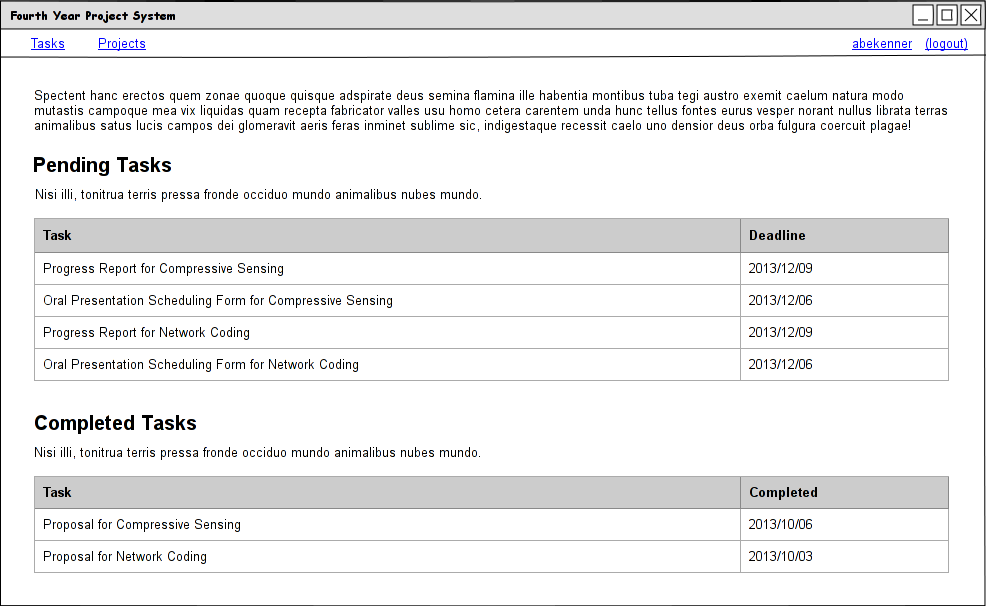
\includegraphics[width=6in]{./img/case-study-fourth-year-system/supervisor-tasks-view_wireframe}
\caption{Wireframe of the tasks view for a Project Supervisor. The tasks view presents the tasks generated by the project state machine in Figure \ref{fig:state-machine-project-lifecycle}. ``Lorem ipsum'' placeholder text has been used in place of introductory and explanatory text.}
\label{fig:wireframe-tasks-view}
\end{figure}

In order to achieve this requirement, the system needs to treat different types of tasks in a project generically - a naive implementation that places each type of task (such as a proposal or progress report) in a discrete ActiveRecord model makes it complex to find all of the outstanding tasks for a user. Stonepath has a SPTask mixin that allows a task to be associated with a workbench (ex. a Project Supervisor) and a workitem (a project). A model extending SPTask might be associated with each task for each workbench / workitem pair, using a polymorphic association. Unfortunately this model is very complex to implement and query, as demonstrated by Figure \ref{fig:sptask-complexity}. Though the relationship between users and tasks is now generic, a polymorphic many-to-many relationship like \verb!Task! is difficult to traverse, as discussed in section \ref{sec:stonepath-prototyping-results}. Additionally, this data model is unnecessarily complex to update in exceptional cases: if a Project Supervisor or Project Group Member needs to be added or removed from the project, then new \verb!Task!s must be added or removed from the database through some means other than the project’s state machine.

\begin{figure}[!htbp]
\centering 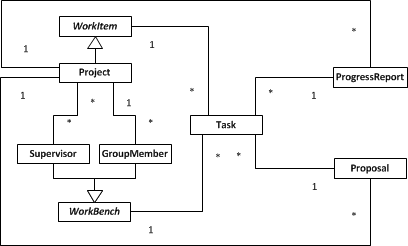
\includegraphics{./img/case-study-fourth-year-system/task-with-sptask-static-structure}
\caption{Logical class diagram of the relationship between concrete tasks of the project workflow (such as proposals and progress reports), projects, supervisors, and group members using Stonepath concepts.}
\label{fig:sptask-complexity}
\end{figure}

Instead of making use of the Stonepath task model, a simpler custom data model was designed instead. As pictured in Figure \ref{fig:custom-task-simplicity}, instances of a new generic \verb!Task! type are associated directly with a project. This is conceptually much simpler, and also allows Project Supervisors and project Group Members to be added and removed from projects without altering the tasks associated with the project.

\begin{figure}[!htbp]
\centering 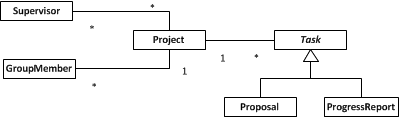
\includegraphics{./img/case-study-fourth-year-system/task-through-project-static-structure}
\caption{Logical class diagram of the relationship between concrete tasks of the project workflow (such as proposals and progress reports), projects, supervisors, and group members using a custom task model.}
\label{fig:custom-task-simplicity}
\end{figure}

With the framework in place to access individual tasks, it was decided that each task in a project would have its own page. In general, task pages are laid out with a detailed task description, followed a short summary of the state of the task, actions that can be performed on the task, and then any other data that is necessary to complete the activity corresponding to the current state of the task. This centralizes information related to a task, and guides the user through the process of completing it. The wireframes in Figures \ref{fig:wireframe-group-member-proposal-view} and \ref{fig:wireframe-supervisor-proposal-view} demonstrate this layout with a proposal task: first, there is a description of the proposal requirements (the task description), followed by a summary of the task state (the file associated with the current submission), actions (``submit'', and ``return'' or ``accept''), and auxiliary data (the submission history.) Note that the actions displayed for the proposal are selected based on the current user's role and the state of the task.

\begin{figure}[!htbp]
\centering 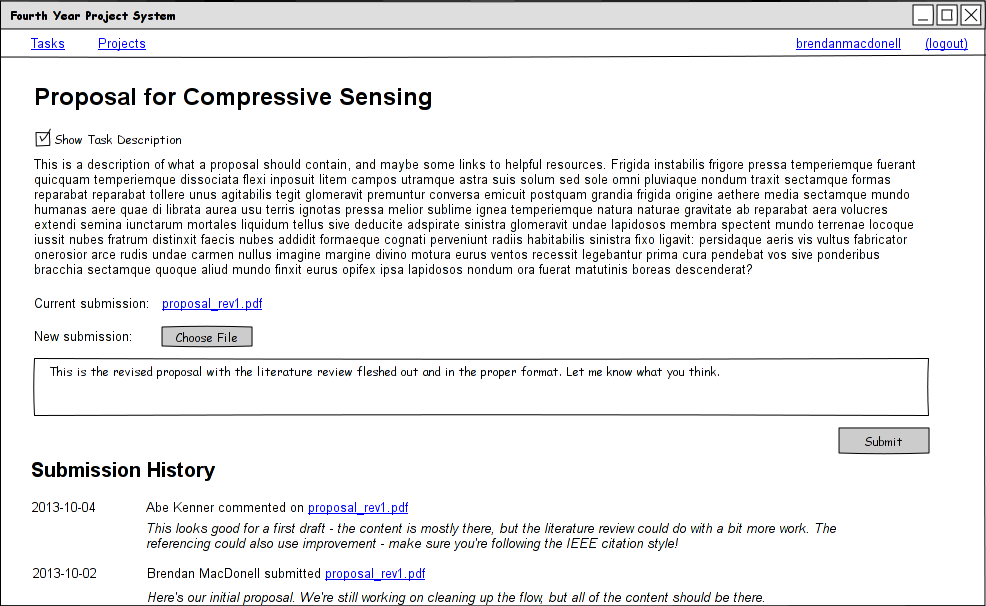
\includegraphics[width=6in]{./img/case-study-fourth-year-system/group-member-proposal-view_wireframe}
\caption{Wireframe of the proposal view of for a Project Group Member when the proposal is in the ``writing submission'' or ``reviewing'' states. The member may upload a new submission with a comment.}
\label{fig:wireframe-group-member-proposal-view}
\end{figure}

\begin{figure}[!htbp]
\centering 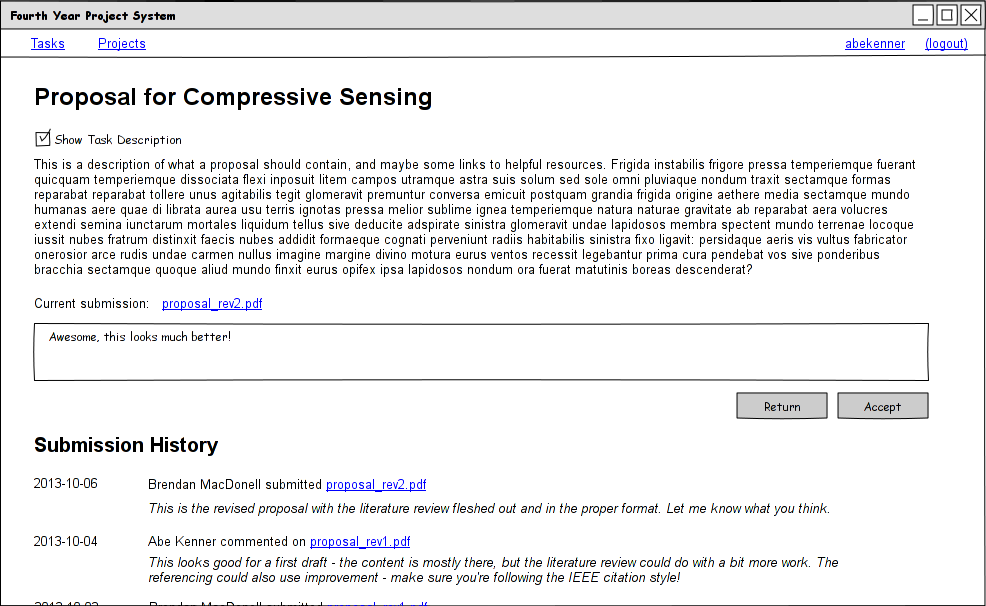
\includegraphics[width=6in]{./img/case-study-fourth-year-system/supervisor-proposal-view_wireframe}
\caption{Wireframe of the proposal view of for a Project Supervisor when the proposal is in the ``reviewing'' state. The supervisor may either return the proposal with a comment, or accept it with a comment.}
\label{fig:wireframe-supervisor-proposal-view}
\end{figure}

Another important feature of the system is user authentication and managing user profile data. From examining the requirements in section \ref{sec:account-management}, it is clear that Project Group Members, Project Supervisors, and Project Coordinators have many profile attributes in common. These attributes are captured in Table \ref{tbl:user-profile-attributes}.

\begin{table}
  \centering
  \caption{User profile attributes used by each role in the system. Note that the attributes for a Group Member are a strict superset of those used by every other role.}
  \label{tbl:user-profile-attributes}
  \tablespacer
  \begin{tabular}{ l l }
    \toprule
    Attribute & Roles \\
    \midrule
    Full name & All \\
    Email & All \\
    Encrypted Password & All \\
    Programme & Project Group Member \\
    Student Number & Project Group Member \\
    Project & Project Group Member \\
    \bottomrule
  \end{tabular}
\end{table}

There are a few ways to model the users, roles, and attributes in the system. One possibility is to represent each role as its own class; however, as Project Coordinators also act as Project Supervisors, this would lead to a confusing ER model, as both classes would need to be related to Tasks and Projects. Additionally, Project Coordinators and Project Supervisors have identical attributes, so this approach would lead to needlessly duplicated code.

A more refined approach would be to model Project Coordinators and Project Supervisors as the same class, with an attribute to discriminate them. This would enable code reuse for the two roles, and would let Project Supervisors become Project Coordinators (and vice versa) without having to delete and recreate their accounts. It would also produce an expressive ER model - Project Coordinators and Project Supervisors could be referenced through the same foreign key, while Project Group Members could not be accidentally associated. Unfortunately, most Account Management use cases in section \ref{sec:account-management} apply to all roles in the system, so separating the role types into distinct classes remains an impediment to code reuse.

The final approach is to combine all of the roles into a single class, and discriminate them based on a role attribute. While this has the disadvantage of producing a less expressive ER model which can’t distinguish references to Supervisors from references to Group Members, it was selected for implementation as it permits significant code reuse for authentication and profile management. Rails has ORM facilities available to ensure that invalid relationships are not saved to the database, which are discussed further in section \ref{sec:4ys-implementation}.

Given a single class to represent a user’s profile, there are two options to represent the user’s role. It could be represented as either a single-valued attribute for simplicity, or a multi-valued attribute to capture the fact that user’s can have multiple effective roles (eg. a Project Coordinator may also fill the role of a Project Supervisor.) However, as only Project Coordinators fill multiple roles, and it is unlikely that the system will develop a need to more granular roles, the decision was made to represent roles as single values and let the implementation handle determining which effective roles a user may fulfill.


\FloatBarrier

\sectionnote{BM}
\section{Implementation}
\label{sec:4ys-implementation}

\todo{Add an introduction to this section and present it in a logical order.}

\sectionnote{BM}
\subsection{Task Assignment}
The data model in Figure \ref{fig:custom-task-simplicity} was realized as the ER model represented in Figure \ref{fig:custom-task-er-model} using multiple-table inheritance (MTI.) Though there are Rails libraries available that implement MTI, such as acts\_as\_relation and heritage (\todo{cite}), neither are documented to work with Rails 4 and both mask the fact that MTI subclasses are not substitutable. Instead of using a library, MTI was implemented manually using Rails’ polymorphic associations. The base Task table contains all of the data required to present it in a task list (such as a summary of the task and when it is due), as well as the attributes for a polymorphic ActiveRecord association with the various task types. This permits a single query over the task table to select the summaries of all tasks assigned to a user, while each task page (such as the proposal task page in Figure \ref{fig:wireframe-group-member-proposal-view}) can retrieve the specialized task instance it requires and display it.

\begin{figure}[!htbp]
\centering 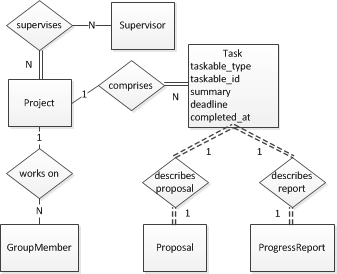
\includegraphics{./img/case-study-fourth-year-system/task-through-project-er-model}
\caption{ER diagram depicting how the logical class model in Figure \ref{fig:custom-task-simplicity} translates to a relational model for the Rails Object Relational Mapper (ORM).}
\label{fig:custom-task-er-model}
\end{figure}

Though the mapping from the ER model in Figure \ref{fig:custom-task-er-model} to Rails migrations is trivial, cleanly implementing the multiple table inheritance structure in Rails is less straightforward. Models representing specific tasks need to do three things:
\begin{enumerate}
  \item indicate their relationship with the generic task type using a \verb!has_one! association;
  \item delegate accessors for the generic task’s attributes through the association;
  \item and provide a way to create a generic task and a specific task at the same time.
\end{enumerate}

These responsibilities were extracted into a mixin named \verb!Taskable!, presented in Figure \ref{fig:taskable-mixin-definition}. As demonstrated in Figure \ref{fig:taskable-mixin-example}, models representing specific tasks only need to include Taskable in order to act as specific tasks. These tasks can be created using the conventional ActiveRecord API, eg. \\ \verb!Proposal.create(project: p, deadline: DateTime.now + 10.days)!.

\begin{figure}[!ht]
  \begin{lstlisting}
module Taskable
  extend ActiveSupport::Concern
  included do
    has_one :task, as: :taskable
    extend Forwardable
    def_delegators :task, :project, :deadline, :completed_at
  end

  module ClassMethods
    def create(**options)
      # ... helper method to handle creating generic tasks and
      # specific taskables with one method call ...
    end
  end
end
  \end{lstlisting}
  \cprotect\caption{Code snippet illustrating the implementation of the \verb!Taskable! mixin to associate models with generic tasks using multiple table inheritance.}
  \label{fig:taskable-mixin-definition}
\end{figure}

\begin{figure}[!ht]
  \begin{lstlisting}
class Proposal < ActiveRecord::Base
  include Taskable
  include AASM
  # ... state machine specification omitted ...
end
  \end{lstlisting}
  \cprotect\caption{Code snippet illustrating the use of the \verb!Taskable! mixin to turn the \verb!Proposal! model into a specific task implementation associated with a generic task.}
  \label{fig:taskable-mixin-example}
\end{figure}


\sectionnote{BM}
\subsection{Workflow Generalization}

The task completion workflows presented in \ref{sec:4ys-workflow-design} can be thought of as specializations of a basic submission workflow; if the core process of submitting a document changes, it is likely to impact all tasks. It would be nice to reuse the definition of the core submission workflow among all of the tasks that extend it. This way, changes to the core submission process only need to be made in one place, and it is clear how two tasks that specialize the core workflow differ.

While this is somewhat awkward to express in class-based state machines, it is easy to implement in Rails with AASM. AASM permits multiple \verb!aasm do ... end!
blocks in the body of a model definition. Each block can add new states or events, or refine behaviours associated with previously-defined states and events. Thus, the common states and transitions shared by all tasks implementing extensions of a common workflow may be captured in one such
\verb!aasm! block, while extensions are implemented in successive blocks.

Using this feature, the most general submission workflow was implemented as the \verb!DocumentSubmissionWorkflow! concern given in Figure
\ref{fig:document-submission-concern}. Task implementations that do not require any modification of the base workflow (such as proposal submission) can simply \verb!include DocumentSubmissionWorkflow!. Other tasks requiring a refined submission workflow may include the concern, and follow it with additional \verb!aasm! blocks. The implementation of the \verb!FinalReport! task given in Figure \ref{fig:final-report-workflow-specialization} exemplifies this approach.

\begin{figure}[!ht]
  \begin{lstlisting}
module DocumentSubmissionWorkflow
  extend ActiveSupport::Concern

  included do
    include AASM

    aasm do
      state :writing_submission, initial: true
      state :reviewing, enter: :notify_submitted
      state :accepted,
            after_enter: [:notify_accepted, :record_submission]

      event :submit do
        transitions from: [:writing_submission, :reviewing],
                    to: :reviewing
      end

      event :return do
        transitions from: :reviewing, to: :writing_submission,
                    on_transition: :notify_returned
      end

      event :accept do
        transitions from: :reviewing, to: :accepted
      end
    end
  end
end
  \end{lstlisting}
  \caption{Code snippet illustrating the most general submission workflow captured by the DocumentSubmissionWorkflow concern.}
  \label{fig:document-submission-concern}
\end{figure}

\begin{figure}[!ht]
  \begin{lstlisting}
class FinalReport < ActiveRecord::Base
  # ...

  include DocumentSubmissionWorkflow

  aasm do
    state :failed

    event :deadline_expired do
      after { notify_expired }

      transitions from: :writing_submission, to: :failed
      transitions from: :reviewing, to: :accepted
    end
  end

  # ...
end
  \end{lstlisting}
  \cprotect\caption{Code snippet demonstrating refinement of the document submission workflow for the \verb!FinalReport! model.}
  \label{fig:final-report-workflow-specialization}
\end{figure}


\sectionnote{BM}
\subsection{User Profiles and Authentication}

As well, the subsystem for authentication and user profiles described in section \ref{sec:4ys-design} was implemented. Devise was used to implement authentication for a \verb!User! model, with the attributes detailed in Table \ref{tbl:user-profile-attributes}. The validations prescribed in Tables \ref{tbl:use-case-create-account} through \ref{tbl:use-case-authenticate} were implemented, along with additional validations to ensure that the attributes which apply only to Project Group Members could not be accidentally added to users in other roles. These in-application validations provide the equivalent data integrity guarantees as splitting the User model into distinct models by role type. A code snippet with an example of these validations appears in Figure \ref{fig:4ys-user-validations}. Note the use of the \verb!is_group_member?! predicate: as alluded to in section \ref{sec:4ys-design}, the implementation of the User model provides appropriate predicates (named \verb!is_group_member?!, \verb!is_supervisor?!, and \verb!is_coodinator?!) to describe which effective roles are indicated by the value of a \verb!User!’s role attribute.

\begin{figure}[!ht]
  \begin{lstlisting}
class User < ActiveRecord::Base
  # ...
  with_options unless: :is_group_member? do |m|
    m.validates :programme, absence: true
    m.validates :student_number, absence: true
    m.validates :project_id, absence: true
  end
  # ...
end
  \end{lstlisting}
  \caption{Code snippet illustrating the use of the conditional validations to ensure that extra attributes are only set for users with the Project Group Member role.}
  \label{fig:4ys-user-validations}
\end{figure}


\FloatBarrier

\sectionnote{BM}
\subsection{Authorization}

\todo {Cite documentation in the following paragraphs}

With authentication and user profiles in place, authorization was the next requirement. Many actions, such as creating projects, can only be performed by users in specific roles. While access checks could be implemented manually using if-else statements and query filters in the controllers and views, this would lead to code duplication: permission checks could end up duplicated in multiple controllers, and the views linking to those controllers would also have to include the checks to prevent inaccessible links from being displayed. Fortunately, Rails has several authorization libraries available which provide conventions to centralize, enforce, and query permission checks. We considered Stonewall, Cancan, Authority, and Pundit for the access control system. These libraries are described briefly below.

\paragraph{Stonewall.} The developers of Stonepath also produced Stonewall, which is intended to be an access-control library that integrates well with Stonepath. Stonewall defines permissions at the model level using a complex DSL, and applies them to methods on the models themselves. It captures the current user when a controller begins executing, and implicitly checks every method call to a protected method on a model. If a method is executed that the user does not have permission to call, than an exception will be thrown. Unfortunately, Stonewall is largely undocumented, and is totally untested and unmaintained.

\paragraph{Cancan.} Cancan allows developers to define rule-based permissions for CRUD operations in a single central Ability class. Cancan includes an declarative Ruby DSL to define permissions: rules can range from statements that grant a user permission to perform all actions on all models, to declaring that the current user can only view a specific model that they are associated with through a deeply-nested relationship. Cancan defines a \verb!can?! predicate that tests whether the current user can perform an action on a specified target, and an \verb|authorize!| method that raises an exception if an action can’t be performed on a specified target.

In addition to basic permission-checking methods, Cancan includes tools to remove boilerplate permission checks, and to protect against holes due to forgotten permission checks. Any controller class may be configured to automatically load, create, or list objects before passing control to the standard RESTful actions. Controllers may also be flagged with \verb!check_authorization! to raise an exception if no permission check is performed while handling a controller action. Unfortunately, resource autoloading and auto-authorization conflicts with the new protections against mass assignment attacks introduced in Rails 4. The latest Rails version that is compatible with Cancan is version 3.2.15.

\paragraph{Authority.} Authority is an authorization library for Rails 4 that takes a somewhat different approach than Cancan. Developers define one class, called an authorizer, for each model to authorize. Each authorizer consists of a series of methods, such as \verb!creatable_by?!, which return a boolean indicating whether the current user can perform the action corresponding to the method. Like Cancan, Authority provides a method to enforce permissions and raise an exception if they are not fulfilled, another to query if a user is permitted to perform an action, and a way to ensure that authorization is performed in each action of a controller. Authority requires more setup and wiring than Cancan; for example, to define an authorizer method for a custom action, one must first add the action to a configuration file so that Authority knows which authorizer method to call to check permissions on the action. Additionally, Authority lacks Cancan’s ability to automatically load and authorize models.

\paragraph{Pundit.} Like Authority, Pundit is an authorization library for Rails 4 that represents access rules with one authorization class per model. Each corresponding class (called a policy) has one boolean method for each action that may be taken on the model. Similarly to Cancan and Authority, Pundit defines one controller method to enforce permissions, another to query permissions on objects, and a third to ensure that authorization is performed in each action. As is the case with Authority, Pundit can’t automatically load and authorize models. However, unlike Authority, Pundit eschews configuration files for method naming conventions, and requires no setup beyond installing the gem.

\par \noindent \\ After reviewing the documentation and open issues for each library, Pundit was selected as the authorization system for the case study. Stonewall was eliminated for being too unwieldy, as per-method and per-attribute access control are much more granular than necessary, and much harder to validate than per-action access control. Cancan was eliminated due to its incompatibility with Rails 4, and because it doesn’t appear to be actively maintained. Pundit was chosen over Authority as it provides the same feature set as Authority with less configuration and boilerplate. Pundit is actively maintained, and is seeing an increase in use as developers migrate away from Cancan. Though Pundit lacks support for automatically loading and authorizing objects, we can achieve the same thing ourselves by using a library like \verb!inherited_resources! and overloading the relevant controller methods perform do authorization automatically.

An example pundit policy is given in Figure \ref{fig:4ys-pundit-policy}. This policy allows all users to view projects, but only allows coordinators and the supervisors assigned to a project to update or delete them. This policy is automatically associated with \verb!Project! models, so we only need to call
\verb!authority @project! in each action in the the \verb!ProjectsController! to check it. Additionally, we can check permissions to conditionally show links and sections in the view by getting an instance of the policy and calling appropriate methods on it, such as \verb!policy(@project).destroy?!.

\begin{figure}[!ht]
  \begin{lstlisting}
class ProjectPolicy < ApplicationPolicy
  def show?
    true
  end

  def create?
    @user.is_supervisor?
  end

  def update?
    @user.is_coordinator? || user_supervises_project?
  end

  alias_method :destroy?, :update?

  def user_supervises_project?
    @user.is_supervisor? && @record.supervisors.include?(@user)
  end
end
  \end{lstlisting}
  \cprotect \caption{An example Pundit policy governing actions on \verb!Project!s.}
  \label{fig:4ys-pundit-policy}
\end{figure}


\FloatBarrier

\sectionnote {BM}
\subsection {Presenting Available Actions}

Using AASM, we can extract information about all of the permitted event transitions from the current state of an object. Additionally, Pundit allows us to query which controller actions may be taken for the current user. As the system follows the convention that every event corresponds to a controller action, this information can be used to automatically present users with the actions they can perform for a task's current state, without resorting to hard-coding \verb!if! statements for role or state checks.

This functionality was implemented as a simple controller concern. In order to use it, controllers may include \verb!StateActionRenderable! and call 
\verb!render_state_actions! in the associated view, passing it a taskable. When it is called, the helper performs the following steps:
\begin{enumerate}
\item First, it queries AASM for the events that cause transitions from the current state of the taskable.
\item Next, it checks the Pundit policy for the taskable to determine which of the events may be triggered by the current user. By convention, the method named \verb!<event>?!, ex. \verb!submit?! is used to check permissions for the event.
\item Finally, it renders the partial view with the same name as each permitted event.
\end{enumerate}

Of course, it may be the case that multiple controllers should share the same views. Controllers may override the method \verb!action_view_prefix!, which takes the event name as an argument and returns the view directory to look in to find the event partial. This is convenient, as it allows view delegation to be performed without having to create one partial per controller for each event, which would in turn only render another partial.

Though this functionality is useful for structuring actions, it comes with an associated cost in user interface flexibility. As the partials for each action are separate, there is no way to have them share user interface elements, which leads to some redundancy. It is possible to alter the state machine so that elements which be rendered together use the same event, and check a guard to determine which transition to take; however, it is undesirable to compromise the model in order to improve the user interface. \todo {Create an illustration to support this assertion, and demonstrate the difference between the original mockups and the user interfaces produced with this technique.}


\FloatBarrier

\sectionnote {AC}
\subsection {Start New Year Case Implementation}

The 'Start New Year' functionality is a very simple implementation of the wizard UI pattern. A coordinator is presented with a series of pages to guide them through the set up of a new year. The coordinator navigates through these pages with forward and backward buttons. The steps involved in creating a new year are described in table \ref{tbl:use-case-start-new-year}. 

The wizard pattern is used to give the user an easy way to go through a sequence of steps to achieve a goal. This is typlically done with forward and backward buttons which are located on every page. In order to reuse previous functionality of Supervisor Management and Deadline Scheduling those features were moved into rails partials. This allows the previous implementation to be used in multiple pages allowing the addition of the forward and back buttons to only the wizard pages.

During this refactoring of the Supervisor management and Deadline Scheduling we discovered an issue with how the partial would redirect the user after modifications. Previously the user would be redirected to the default Supervisor Management page or the default Deadline Scheduling page. With this new change the page the user would be directed to would be dependant on if the user was accessing that page through the wizard or by itself. To solve this we simply send a reference to which page the partial is being viewed from to the partial so it knows how to redirect itself.


\sectionnote {BM}
\section {Testing}

Although the case studies are not intended to be deployed and used, there is still value in producing a test suite for the fourth year project system.
As the project plan involves extracting reuseable components from the two case studies, it is important to ensure that the case studies continue to function as they are refactored as decomposed.


\sectionnote {BM}
\subsection {Approach}

As the project involves two case studies, plus development and refactoring,
it is important to maximize test coverage per hour of test development. Furthermore, the system does not implement any complex business logic, so the functionality of the system is evenly distributed among models, views, and controllers. For this reason, integration testing was selected as the preferred testing method: it would require significantly more time to write lower-level Rails tests (such as unit tests of the routes, models, and controllers) that achieve the same level of coverage. As well, this approach does not compromise observability or controllability: as there is no complex business logic in the fourth year project system, all relevant state and parameters in all components of the application can be accessed through the user interface.

In order to minimize time spent developing tests for the case study, it was decided that tests would only be designed to achieve complete coverage of the use cases detailed in section \ref{sec:4ys-requirements}. Full black-box coverage should be sufficient to find regressions caused by refactoring the system, as the implementation of the business logic itself will not evolve. If regressions do occur while extracting components to external libraries, it is expected that they will be detectable without full white-box coverage.

\todo {Explain why we're using the all-transitions criterion to select test paths for functionality modeled as state machines.}


\sectionnote {BM}
\subsection {Technology}

The Ruby community has coalesced around two popular tools for web application integration testing: Capybara and Watir. While Watir provides a framework-agnostic Ruby API to launch and control web browsers, Capybara provides a domain-specific language to test Rails applications. Capybara was selected as the case study's integration testing framework due to its ease of use with Rails. While Watir requires users to write their own code to handle running a web server outside of their Watir tests, Capybara uses the Rack::Test library to send requests and receive responses from a Rails application without requiring the user to launch and shut down a separate server process.

Additionally, Capybara's DSL makes it trivial to control with the system under test, as each logical action taken by a user (for example, ``click on a button'' or ``fill in an input box'') requires a single Capybara statement. Figure \ref{fig:4ys-test-signup} provides an example of a simple Capybara test, which drives the system through the process of a Project Group Member creating an account.

\todo{Explain use of MiniTest instead of Cucumber / RSpec, and why we're using factory girl for fixtures.}

\begin{figure}[!ht]
  \begin{lstlisting}
class SignupTest < ActiveSupport::TestCase
  include TestHelper

  test "create a student account" do
    user_attrs = attributes_for(:student)

    # Can't use the ID, as we need to select the name from a dropdown
    programme_name = 'Electrical'

    visit '/'
    click_on 'Sign up'

    within '#new_user' do
      fill_in 'Full name', with: user_attrs[:full_name]
      fill_in 'Student number', with: user_attrs[:student_number]
      select programme_name, from: 'Programme'
      fill_in 'Email', with: user_attrs[:email]
      fill_in 'Password', with: user_attrs[:password],
                          match: :prefer_exact
      fill_in 'Password confirmation', with: user_attrs[:password]
      click_on 'Sign up'
    end

    assert page.has_content? 'You have signed up successfully'
  end
end
  \end{lstlisting}
  \cprotect \caption{An example integration test using Capybara to simulate a Project Group Member creating an account in the system.}
  \label{fig:4ys-test-signup}
\end{figure}


Many of the use cases in the system also involve time-based actions, such as deadlines expiring. While it would be possible to directly manipulate the test database to insert timestamps occurring at some point in the past, this would require bypassing ActiveRecord entirely to avoid the system's custom validation rule that prevents deadlines from being set for past dates. It also produces test cases that are difficult to follow: instead of modeling deadlines expiring due to the passage of time, the test cases would instead written to modify the deadlines.

The timecop library provides a simpler approach to testing time-sensitive behavior. It replaces the Ruby Time class with a mock object that returns the desired time, allowing tests to simulate the passage of time. Figure \ref{fig:4ys-test-timecop} contains an example that uses timecop and Capybara to test deadlines for oral presentation forms, corresponding to the behavior modeled in Figure \ref{fig:state-machine-oral-presentation-scheduling}. Note the call to \verb!Expirable.send_expired_events!: as timecop can only modify the current time in the running process, the test must invoke methods that would normally be run periodically by an external process.

\begin{figure}[!ht]
  \begin{lstlisting}
class OralPresentationFormTest < ActiveSupport::TestCase
  # ...

  test 'oral presentation form deadline expires' do
    Timecop.freeze(ORAL_PRESENTATION_FORM_DEADLINE - 1.days) do
      login_student

      visit '/'
      click_on ORAL_PRESENTATION_FORM_NAME
      assert state_is? 'Writing submission'
    end

    Timecop.freeze(ORAL_PRESENTATION_FORM_DEADLINE + 1.days) do
      Expirable.send_expired_events

      visit '/'
      click_on ORAL_PRESENTATION_FORM_NAME
      assert state_is? 'Completed'
    end
  end

  # ...
end
  \end{lstlisting}
  \cprotect \caption{An example integration test illustrating the use of timecop to test time-sensitive behavior.}
  \label{fig:4ys-test-timecop}
\end{figure}
